\documentclass[aspectratio=169]{beamer}
\geometry{paperwidth=160mm,paperheight=100mm}
\usepackage{beamerthemesidebar}
\usepackage{hyperref}
\usepackage{color}
\usepackage{multimedia}
\usepackage{colortbl}
\usepackage{amsmath}
\usepackage{empheq}
\usepackage{cancel}
\usepackage{amssymb}
\usepackage{amsfonts}
\usepackage{lipsum}
\usepackage{tcolorbox}
\usepackage{tabularx}
\usepackage{caption}
\usepackage{bm}

\setbeamersize{sidebar width right=0pt}
\setbeamertemplate{footline}[frame number]
%
\definecolor{orange}{RGB}{250,167,12}
\definecolor{yellow}{RGB}{246,250,12}
\definecolor{green}{RGB}{128,238,1}
\definecolor{black}{RGB}{0,0,0}
\definecolor{blue}{RGB}{0,0,255}
\definecolor{red}{RGB}{255,0,0}
\definecolor{sepia}{RGB}{94,38,18}
\newcommand{\ve}[1]{{\rm\bf {#1}}}
\newcommand{\q}[1]{\textcolor{blue}{#1}}
\newcommand{\blue}[1]{\textcolor{blue}{#1}}
\newcommand{\sepia}[1]{\textcolor{sepia}{#1}}
\newcommand{\red}[1]{\textcolor{red}{#1}}
\newcommand{\green}[1]{\textcolor{green}{#1}}
\newcommand{\yellow}[1]{\textcolor{yellow}{#1}}
\newcommand{\orange}[1]{\textcolor{orange}{#1}}
\definecolor{burlywood}{RGB}{255,211,155}
\definecolor{chocolate}{RGB}{255,127,36}
\definecolor{tan}{RGB}{210,180,140}
%
\def\onethird{{\textstyle{1\over3}}}
\def\twothirds{{\textstyle{2\over3}}}
\def\onehalf{{\textstyle{1\over2}}}
\def\threehalfs{{\textstyle{3\over2}}}
%
\newcommand{\pd}{\partial}
\newcommand{\aMLT}{\alpha_{\rm MLT}}
\newcommand{\Fconv}{F_{\rm conv}}
\newcommand{\Hp}{H_p}
%
\title{Theoretical Astrophysics I: Physics of Sun and Stars\\
Lecture 4: Convective energy transport}
\author{\texorpdfstring{\sepia{Petri K\"{a}pyl\"{a} Ivan Mili\'{c}}\newline\blue{\url{pkapyla, milic@leibniz-kis.de}}}{}}
\institute{Institut f\"ur Sonnenphysik - KIS, Freiburg}
\date{\today}
%
\begin{document}
\frame{\titlepage}

\section{Equation of state}
\frame{
	\frametitle{Energy transport mechanisms in stars}
	\begin{itemize}
		\item Radiation: photons transport the energy. Mean
                  free path is very short and this can be modeled as a
                  diffusion process down the temperature gradient, i.e.,
                  \begin{equation}
                    {\bf F}_{\rm rad} = - K_{\rm rad} \bm\nabla T,\label{equ:Frad}
                  \end{equation}
                  where $K_{\rm rad}$ is the radiative conductivity.
		\item Conduction: heat is transported because of
                  collisions of particles. Analogous to
                  \ref{equ:Frad}, this is written as
                  \begin{equation}
                    {\bf F}_{\rm cd} = - K_{\rm cd} \bm\nabla T.\label{equ:Fcond}
                  \end{equation}
                  Typically $K_{\rm rad} \gg K_{\rm cd}$ (\blue{Except
                    where?}).
		\item Convection: gas is opaque to radiation, becomes
                  \emph{unstable}, and fluid motions transport the
                  energy. This leads to very complicated dynamics and
                  cannot in general be represented in equally simple
                  terms as radiation or conduction.
	\end{itemize}
}
%
\frame{
\frametitle{Intuitive picture of convective instability}
\begin{minipage}{0.4\linewidth}
\begin{itemize}
	\item Consider a fluid element with density $\rho_1$ and
          pressure $p_1$ displaced upward to a level where
          $\rho=\rho_2$ and $p=p_2$.
	\item If the density inside the element ($\rho_\star$) is
          larger (smaller) than the ambient density, it is pulled back
          (continues to accelerate).
        \item Assumption: no heat exchange between fluid element and
          the surroundings.
\end{itemize}
\end{minipage}
\hfill
\begin{minipage}{0.59\linewidth}
\begin{figure}
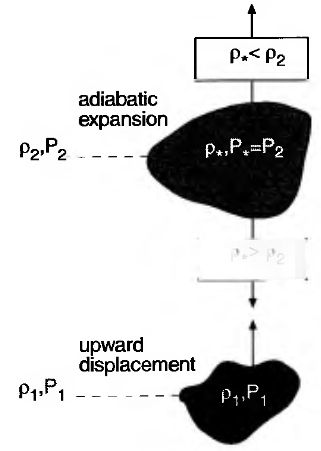
\includegraphics[width=3.5cm]{figures/convective_blobs.png}
\caption*{Source: Prialnik}
\end{figure}
\end{minipage}
%% Convection leads to \emph{circulation} of matter (but no net mass
%% transport).
}
%
%
\frame{
\frametitle{Schwarzschild criterion}
\begin{minipage}{0.4\linewidth}
\begin{itemize}
	\item Consider the atmospheres A, S, and S': the stably
          stratified case corresponds to S', where
          \begin{equation}
            \frac{\pd p}{\pd \rho} < \left(\frac{\pd p}{\pd \rho}\right)_{\rm a}\label{equ:Sch1}
          \end{equation}
%	\item For an adiabatic process $p = K_{\rm a} \rho^{\gamma_{\rm a}}$
        \item This form is not particularly useful so we will recast
          it in terms of a temperature gradient.
        \item Recall the 1st law of thermodynamics:
          \begin{equation}
            dQ = du + pdV.
          \end{equation}
\end{itemize}
\end{minipage}
\hfill
\begin{minipage}{0.59\linewidth}
\begin{figure}
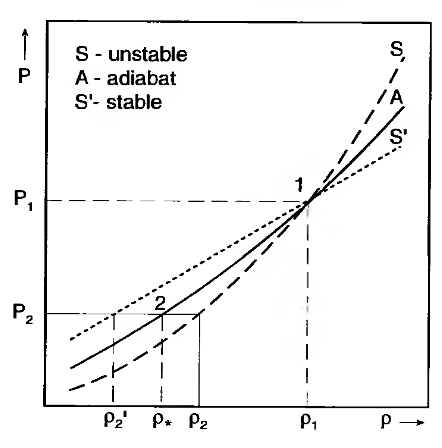
\includegraphics[width=6cm]{figures/pvsrho_convection.png}
\caption*{Source: Prialnik}
\end{figure}
\end{minipage}
}
%
\frame{
\frametitle{Schwarzschild criterion}

\begin{itemize}
\item The ideal gas equation can be written as:
  \begin{equation}
    p = \frac{{\cal R}}{\mu} \rho T = (c_p - c_V) \rho T,
  \end{equation}
  where $c_p$ and $c_V$ are specific heat capacities at constant
  pressure and at constant volume. Their ratio is $\gamma = c_p/c_V =
  5/3$.
\item Furthermore, with the internal energy $u = c_V T$ this becomes
  \begin{equation}
    p = \frac{{\cal R}}{\mu} \rho T = (\gamma - 1) \rho u,\ \ \mbox{and} \ \ u = \frac{1}{\gamma-1} \frac{p}{\rho}. 
  \end{equation}
\end{itemize}
}
%
\frame{
\frametitle{Schwarzschild criterion}

\begin{itemize}
\item For an adiabatic process $dQ = 0$. Furthermore, the specific
  volume is $V = \rho^{-1}$, and $dV = -d\rho/\rho^2$. Thus,
  \begin{equation}
    \frac{1}{\gamma-1} \left(\frac{dp}{\rho} - p \frac{d\rho}{\rho^2} \right) - p \frac{d\rho}{\rho^2} = 0.
  \end{equation}
  \begin{equation}
    \frac{1}{\gamma-1} \left(\frac{dp}{p} - \frac{d\rho}{\rho} \right) - \frac{d\rho}{\rho} = 0.
  \end{equation}
  \begin{equation}
    \frac{1}{\gamma-1} \left(\frac{\rho}{p}\frac{dp}{d\rho} - 1 \right) - 1 = 0.
  \end{equation}
  \begin{equation}
    \frac{\rho}{p}\frac{dp}{d\rho} = \left(\frac{\rho}{p}\frac{dp}{d\rho}\right)_{\rm a} = 1 + (\gamma - 1) = \gamma.
  \end{equation}
\end{itemize}
}
%
\frame{
\frametitle{Schwarzschild criterion}

\begin{itemize}
\item Going back to Eq.~(\ref{equ:Sch1}) we can write:
  \begin{equation}
    \frac{\rho}{p}\frac{dp}{d\rho} < \left(\frac{\rho}{p}\frac{dp}{d\rho}\right)_{\rm a} = \gamma.\label{equ:adia1}
  \end{equation}
\item For an ideal gas
  \begin{equation}
    \frac{dp}{p} = \frac{d\rho}{\rho} + \frac{dT}{T}.
  \end{equation}
\item Multiply by $p/dp$, make use of Eq.~(\ref{equ:adia1}) and define
  $\nabla_{\rm a}$:
  \begin{equation}
    1 = \left(\frac{p}{\rho}\frac{d\rho}{dp} + \frac{p}{T} \frac{dT}{dp}\right)_{\rm a} \equiv \frac{1}{\gamma} + \nabla_{\rm a},
  \end{equation}
  or:
  \begin{equation}
    \nabla_{\rm a} = 1 - \frac{1}{\gamma} = \frac{\gamma-1}{\gamma}.
  \end{equation}
\end{itemize}
}
\frame{
\frametitle{Schwarzschild criterion}

\begin{itemize}
\item Extending the definition of $\nabla$ to the general case 
  \begin{equation}
    \nabla \equiv \frac{p}{T}\frac{dT}{dp},
  \end{equation}
  we can rewrite the stability condition (\ref{equ:adia1}) as
  \begin{equation}
    \nabla < \nabla_{\rm a}.
  \end{equation}
\item Sometimes the quantity $\Delta\nabla = \nabla - \nabla_{\rm a}$
  (superadiabaticity) is used to denoted whether a layer is
  convectively stable or not.
\item In stellar convection zones (apart from the near-surface layes)
  $\Delta \nabla$ is very small, e.g., ${\cal O}(10^{-3}\ldots
  10^{-4})$ in the Sun.
\end{itemize}
}
%
\frame{
\frametitle{Schwarzschild criterion -- reflection}
\begin{itemize}
\item Violation of Schwarzschild criterion is necessary but not
  sufficient condition for convection to occur (\blue{Why?})
\end{itemize}
}
%
\frame{
\frametitle{Schwarzschild criterion -- reflection}
\begin{itemize}
\item Violation of Schwarzschild criterion is necessary but not
  sufficient condition for convection to occur (\blue{Why?})
\item Internal friction in the gas was been neglected $\rightarrow$ in
  reality $\Delta \nabla$ has to exceed a finite value $\Delta
  \nabla_{\rm min}$ (which depends on $T$, $\rho$, rotation, magnetic
  fields, etc.) for convection to ensue.
\item Typically this is represented by a Rayleigh number which is a
  ratio of convective transport to diffusive transport:
  \begin{equation}
    {\rm Ra} = \frac{g d^4}{\nu\chi H_p} \Delta\nabla,
  \end{equation}
  where $g = GM/r^2$, $\nu$ is the kinematic viscosity, $\chi = K_{\rm
    rad}/\rho c_p$ is the radiative diffusivity, and $H_p$ is the
  pressure scale height.
\item Critical value for free convection is ${\rm Ra}_{\rm c} \approx
  1500$. In the Sun, ${\rm Ra} \approx 10^{20}$.
\end{itemize}
}
%
\frame{
\frametitle{Mixing length theory}

\begin{itemize}
\item Assume discrete gas elements that move a vertical distance
  $\ell$ before dissolving.
\item This distance is called the \emph{mixing length}, and is given
  by $\ell = \aMLT \Hp$, where $\aMLT = {\cal O}(1)$.
\item Consider the convective energy flux (unit: W/m$^2$) is:
  \begin{equation}
    \Fconv = c_p \rho u T',\label{equ:Fconv}
  \end{equation}
  where $u$ is the convective velocity, and $T' = T - \overline{T}$.
\end{itemize}
}
%
\frame{
\frametitle{Mixing length theory}

\begin{itemize}
\item Average (squared) convective velocity is
  \begin{equation}
    u^2 = g \delta (\nabla-\nabla_{\rm e}) \frac{\ell^2}{8h_p}.
  \end{equation}
\end{itemize}
}
%
%
\frame{
\frametitle{Estimates of convective velocity and temperature fluctuations}

\begin{itemize}
\item Velocity from convective flux, Eq.~(\ref{equ:Fconv})
  \begin{equation}
    u = \left( \frac{F}{\rho} \right)^{1/3}
  \end{equation}
\end{itemize}
}
%
\end{document}



